\documentclass{beamer}
\usetheme{metropolis} 
\usecolortheme{rose}

\usepackage{xcolor}
\usepackage[utf8]{inputenc}
\usepackage{hyphenat}
\usepackage[russian,english]{babel}          % Use metropolis theme
\usepackage{wrapfig}

\setbeamertemplate{footline}[frame number] % указывает на каждой странице общее количество страниц

% Указывайте все новые термины в \termdef команде. А уже известные ранее или из других курсов в \term
\newcommand{\termdef}[1]{\textbf{\textit{#1}}}
\newcommand{\term}{\textit}
% Диалог с аудиторией.
\newcommand{\auditorium}[1]{\color{red}{\textbf{#1}}}
% \setbeamercolor{auditorium}{fg=red}

\title{Лекция 2, часть I. Классификация. Основные понятия.}
% \date{\today}
\date{24 сентября 2019}
\author{Павел Владимирович Слипенчук}
\institute{Москва, МГТУ им.Бауманка,\\ каф.ИУ-8, КИБ}
% \titlegraphic{\includegraphics[width=2cm]{logo_ur.jpg}}
\titlegraphic{\small \href{https://github.com/kib-courses/dsis}{Data Science для решения задач информационной безопасности}}

\begin{document}
  \maketitle
    
  \begin{frame}{План лекции}
    \begin{enumerate}
	\item \nameref{section:classification_defs}
	\item \nameref{section:precision_recall_defs}
	\item \nameref{section:all_of_them}
	\end{enumerate}
 \end{frame}
    
  \section{Признак. Вектор признаков Классы. Обучающая и тестовая выборки. Задача классификации, классификатор(оценщик)}\label{section:classification_defs}
  
  \begin{frame}{Признак, вектор, класс}
    \termdef{Признак} $x_i$-- определенное значение. Категориальное, сравнимое, или числовое: целочисленное, булевое, или дробное.
    
    \termdef{Вектор признаков} $\bold x = (x_1, x_2, ... x_n)$ -- вектор, каждое значение которого является \term{признаком}. 
  	
  	\termdef{Класс} (метка) $y$ -- значение (как правило целочисленное), присваиваемое какому-либо вектору признаков: $ y \mapsto \bold x$
  	
  	\auditorium{А в чем физический смысл?}
  \end{frame}
  
  \begin{frame}{Пример}\label{frame:class_feature_vector_example}
  \begin{itemize}
  	 \item $x_1$ -- сумма транзакции [в рублях]
  	 \item $x_2$ -- возраст клиента [в годах]
  	 \item $x_3$ -- пол клиента [булевый: 1 -- мужской, 0 -- женский]
  	 \item $x_4$ -- MCC код\footnote{\termdef{Merchant Category Code} -- номер деятельности компании при осуществлении безналичной оплаты. Например \textbf{1731} означает оплату за электроэнергию, \textbf{3137} -- покупка авиабилетов, \textbf{4121} -- такси}
  	 \item  $y=1$ -- операция мошенническая (фродовая);  $y=0$ -- легитимная.
  \end{itemize}
  \begin{center}\small \begin{tabular}{ l l }
  	$0 \mapsto (3234, 25, 1, 1731) $ &  $0 \mapsto (2540, 55, 0, 1731)$ \\
  	$1 \mapsto (18400, 45, 0, 3137)$ & $0 \mapsto (2540, 55, 0, 1731)$  \\
  	$1 \mapsto (903, 19, 0, 4121)$  & $0 \mapsto (1875, 45, 0, 4121)$  \\
  	$0 \mapsto (854, 21, 1, 4121)$  & $1 \mapsto (702, 21, 0, 4121)$  \\
  	$1 \mapsto (903, 19, 0, 4121)$  & $0 \mapsto (1875, 45, 0, 4121)$  \\
  	$0 \mapsto (28400, 41, 1, 3137)$ & $0 \mapsto (25040, 55, 0, 1731)$  \\
  \end{tabular}\end{center}
  \end{frame}
  
  \begin{frame}
   \begin{block}{Замечание}
	  В отличие от таблицы, представленной на слайде №\ref{frame:class_feature_vector_example},
	  в данных на реальных задачах \term{вектор признаков} может состоять из $~200$ и более признаков:
	  $\bold x = (x_1, x_2, ..., x_{200}, ...)$
  \end{block}
   \end{frame}

  \begin{frame}
\begin{block}{Замечание}
	Иногда можно встретить ещё два понятия: \term{характеристика} и \term{контрибутор}.
	
	\termdef{Характеристика} -- это какая-либо информация из которой можно получить один
	или более признаков.
	
	\termdef{Контрибутор} (контрибьютер) -- это совокупность признаков (возможно один),
	который вносит определённый вклад в скоринговую модель. 
	
	Однако можно считать эти термины устаревшими, так как
	\term{Feature Extraction} ввело понятие \term{<<сырые данные>>} (raw data)
	и убило понятие характеристика; 
	а ансамбли сделали ненужным термин контрибутор.
\end{block}
\end{frame}

  
  \begin{frame}{Функция высшего порядка}
  \termdef{Функция высшего порядка} -- это функция, принимающая в качестве аргументов хотя бы одну другую функцию и/или возвращающая в качестве выхода функцию.
  
  \auditorium{ДЗ. см.так же:}
  \begin{enumerate}
  	\item \termdef{функциональное программирование}
  	\item \termdef{декоратор}, \termdef{фабрика декораторов}
  \end{enumerate}
  
  \end{frame}
  
  \begin{frame}{Классификация. Постановка задачи}\label{frame:classification_def}
  	\small
  	Определим \term{неупорядоченную совокупность}:
  	\begin{equation}\label{eq:def_fit_sample}
  	U_{fit} = \left\{ y \mapsto \bold x  \right\}
  	\end{equation}
  	где $y$ -- это \term{класс},
  	а $\bold x$ -- это \term{вектор признаков}.
  	Множество \eqref{eq:def_fit_sample} будем называть \termdef{обучающей выборкой}.
 
  	Функцию, отображающую вектор $\bold x$ в значения на интервале $[0, 1]$ будем 
  	называть \termdef{функцией скоринга}:
  	\begin{equation}\label{eq:score_def}
  	\hat{y} := score( \bold x); \hat{y} \in [0, 1]
  	\end{equation}
  	Значение $\hat{y}$ называют \termdef{откликом} \term{вектора признаков} $\bold x$.
  	
  	\termdef{Обучением} (в задаче классификации) будем называть процесс получения 
  	\term{функции скоринга}\eqref{eq:score_def} 
  	из 
  	\term{обучающей выборки}\eqref{eq:def_fit_sample}.
  	Таким образом можно определить \term{функцию высшего порядка} $fit$:
  	\begin{equation}\label{eq:fit_def}
  	score := fit (U_{fit}) 
  	\end{equation}
  \end{frame}


	\begin{frame}
	Как правило множество $U_{fit}$ задается парой:
	\begin{equation}
		U_{fit} := (\bold X, \bold y) 
	\end{equation}
	где $\bold X$ и $\bold y$ -- это \textbf{упорядоченные} совокупности (списки)
	из \term{векторов признаков} $\bold  x$ и соответствующих им \term{классов} $y$. 
	
	% См.например:
	%\url{https://scikit-learn.org/stable/modules/generated/sklearn.ensemble.RandomForestClassifier.html\#sklearn.ensemble.RandomForestClassifier.fit}
	
	То есть:
	\begin{equation}
	\bold X \stackrel{def}{=} \left( 
	(x_1^1, x_2^1, ..., x_n^1),
	(x_1^2, x_2^2, ..., x_n^2),
	... ,
	(x_1^m, x_2^m, ..., x_n^m)
	\right)
	\end{equation}
	\begin{equation}
	\bold y \stackrel{def}{=} (y^1, y^2, ..., y^m) 
	\end{equation}
	где верхние цифры -- это индексы, а не степени.
	\end{frame}


	  
	\begin{frame}{Классификация}
	\small
	Функция $fit$ (cм. \eqref{eq:fit_def} на слайде №\ref{frame:classification_def}) возвращает функцию $score$, которая размечает каждую точку пространства признаков на величину от 0 до 1. Чем ближе эта величина к 1, тем <<более вероятно>> что это класс 1, чем ближе к 0 -- тем более вероятно что класс 0.
	\begin{center}
		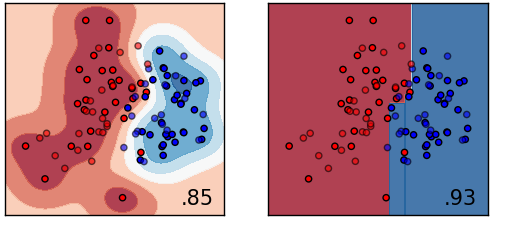
\includegraphics[width=7.5cm]{../pic/classification_example.png}\centering
	\end{center}
    \begin{block}{Замечание}
    Иногда для удобства fit возвращает не в диапазоне $[0, 1]$,
    а в диапазоне $[-1, 1]$.
    \end{block}
\end{frame}


 \begin{frame}
	 \begin{block}{Замечание}
	 	$U_{fit}$ в общем случае это именно неупорядоченная совокупность, а не множество. Во множестве ни один элемент не может быть более одного раза, а в неупорядоченной совокупности -- может. Для простоты в дальнейшем 	$U_{fit}$ будем называть множеством.
	 \end{block}
	\begin{block}{Замечание}
		Иногда функция $fit$ представляет собой \term{ленивое вычисление}\footnote{
		\termdef{Ленивые вычисления} (lazy evaluation, отложенные вычисления) -- 
		метод программной разработки функций, в которой вычисления откладывают до тех пор,
		пока не понадобится их результат.
		} и выдаёт $score$ почти мгновенно. И уже для каждого конкретного $\bold x$ функция
		$score(\bold x)$ рассчитывает \term{отклик} $\hat{y}$ на основании 
		\term{обучающей выборки} \term{} $U_{fit}$
	\end{block}
   \end{frame}
  
	\begin{frame}
	Без использования алгоритмов машинного обучения, функцию $score$ необходимо разрабатывать 
	<<вручную>>. Пример слайда №\ref{frame:class_feature_vector_example}:
	\begin{center}\small \begin{tabular}{ l l }
			$0 \mapsto (3234, 25, 1, 1731) $ &  $0 \mapsto (2540, 55, 0, 1731)$ \\
			$1 \mapsto (18400, 45, 0, 3137)$ & $0 \mapsto (2540, 55, 0, 1731)$  \\
			$1 \mapsto (903, 19, 0, 4121)$  & $0 \mapsto (1875, 45, 0, 4121)$  \\
			$0 \mapsto (854, 21, 1, 4121)$  & $1 \mapsto (702, 21, 0, 4121)$  \\
			$1 \mapsto (903, 19, 0, 4121)$  & $0 \mapsto (1875, 45, 0, 4121)$  \\
			$0 \mapsto (28400, 41, 1, 3137)$ & $0 \mapsto (25040, 55, 0, 1731)$  \\
	\end{tabular}\end{center}
	
	Можно задать функцию $score$ следующим способом:
	\begin{equation}\label{eq:score_example}
		score := \left\{ 
			\begin{array}
			[c]{ll}%
			0, ~$если$~ x_3 = 1 \vee x_4 = 1731
			\\
			0.6667, ~$если$~ x_3 = 0  \wedge x_4 \neq 1731
			\end{array}
		\right.
	\end{equation}

	\end{frame}

	\begin{frame}{Переобучение (Переподгонка, Overfitting)}
	\termdef{Переобучение} -- эффект построенной модели (функция $score$), 
	при котором на тестовой выборке модель работает существенно хуже.
	\begin{wrapfigure}{l}{0.4\textwidth}
	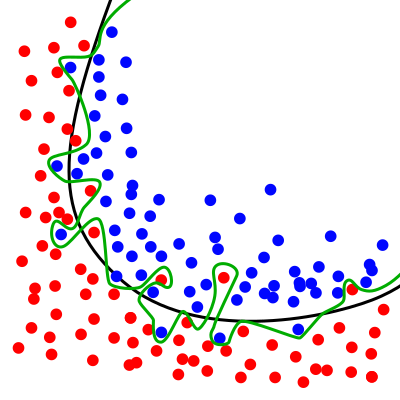
\includegraphics[width=4cm]{../pic/overfitting_example.png}\centering
	% \caption{Пример переобучения и нормального обучения}
	\end{wrapfigure}	
	Это связано с тем, что при построении модели («в процессе обучения») в обучающей выборке обнаруживаются некоторые случайные закономерности, которые отсутствуют в генеральной совокупности.
	\end{frame}
   	
   	\begin{frame}{Пример переобучения}
   	В примере \eqref{eq:score_example} у нас никогда не бывает мошенничества если клиент является 
   	мужчиной ($x_3=1$):
   	 \begin{equation*}
   	score := \left\{ 
   	\begin{array}
   	[c]{ll}%
   	0, ~$если$~ x_3 = 1 \vee x_4 = 1731
   	\\
   	0.6667, ~$если$~ x_3 = 0  \wedge x_4 \neq 1731
   	\end{array}
   	\right.
   	\end{equation*}
   	Однако это абсурд! Просто у нас такая выборка:
   \begin{center}\small \begin{tabular}{ l l }
   		$0 \mapsto (3234, 25, 1, 1731) $ &  $0 \mapsto (2540, 55, 0, 1731)$ \\
   		$1 \mapsto (18400, 45, 0, 3137)$ & $0 \mapsto (2540, 55, 0, 1731)$  \\
   		$1 \mapsto (903, 19, 0, 4121)$  & $0 \mapsto (1875, 45, 0, 4121)$  \\
   		$0 \mapsto (854, 21, 1, 4121)$  & $1 \mapsto (702, 21, 0, 4121)$  \\
   		$1 \mapsto (903, 19, 0, 4121)$  & $0 \mapsto (1875, 45, 0, 4121)$  \\
   		$0 \mapsto (28400, 41, 1, 3137)$ & $0 \mapsto (25040, 55, 0, 1731)$  \\
   \end{tabular}\end{center}
	\end{frame}
   
   \begin{frame}{Обучение с подкреплением, reinforcement learning (Дообучение, Refitting)}
  	Есть первоначальная обучающая выборка: 
   \begin{equation*}
    U_{fit} = \left\{ y \mapsto \bold x  \right\}
   \end{equation*}
 	Первоначальное обучение:
  \begin{equation*}
  score_1 := fit (U_{fit}) 
  \end{equation*} 
  	В дальнейшем при получении нового множества $\hat U_{fit}$ (возможно состоящее из одного элемента)
  	мы дообучаем систему:
  	\begin{equation}
  	score_{i+1} := refit (\hat U_{fit}, score_{i}) 
  	\end{equation} 
   	Таким образом функция $score_i$ заменяется на новую функцию $score_{i+1}$.
   \end{frame}

	\section{Тестовая выборка. Отсечка. tp, tn, fp, fn. Полнота и точность.}\label{section:precision_recall_defs}

	\begin{frame}
	Итак, у нас построена $score$ каким-либо алгоритмом машинного обучения. 
	Пока оставим за скобками как этот алгоритм построен. Это <<чёрный ящик>>.
		
	\begin{center}
	
\includegraphics[width=5cm]{../pic/magic_box.png}\centering
	\end{center}
	\end{frame}

	

	\begin{frame}{Тестовая выборка}
	После того как мы задали функцию оценщика ($score$)
	необходимо как-то оценить качество этой функции.
	
	Для этого мы выбираем другую выборку $U_{test}$ и для каждого $\bold x \in U_{test}$ 
	находим $\hat y$. 
	
	Таким образом можно задать совокупность пар:
	\begin{equation}
	\{(y, \hat y)\} := \left\{ (y, \hat y)~~\forall (\bold x, y) \in U_{test} : \hat y := score(\bold x) \right\} 
	\end{equation}
	
	После того, как мы задали какую либо отсечку ($offset$), мы каждую пару $(y, \hat y)$ можем отнести к одному из четырёх 
	событий: \textbf{true positive (tp), true negative (tn), false positive (fp), false negative (fn)}.
		
	\auditorium{Вспоминаем первую лекцию. Что такое полнота и точность?}
	\end{frame}

	\begin{frame}
	Просмотрим для определённой отсечки $offset$
	множество ${y, \hat y}$. 
	Если $\hat y \geqslant offset$ -- то это \textbf{positive}, 
	если $\hat y < offset$ -- то это \textbf{negative}.
	
	Если $y=0$ и \textbf{negative} или $y=1$ и \textbf{positive}, то это \textbf{true} negative/positive.
	Иначе \textbf{false}  negative/positive.
	
	Определим величины:
	\begin{enumerate}
		\item $ctp$ (count true positive) -- количество событий true positive (tp);
		\item $cfp$ (count false positive) -- количество событий false positive (fp);
		\item $ctn$ (count true negative) -- количество событий true positive (tn);
		\item $cfn$ (count false negative) -- количество событий false negative (fn).
	\end{enumerate}
	\end{frame}

	\begin{frame}{Вопрос на засыпку}
	Верно ли, что полноту ($\Pi$) и точность ($T$) можно определить с помощью формул?:
	\begin{equation*}
	\Pi = \frac{ctp}{ctp + cfn}
	\end{equation*}
	\begin{equation*}
	T = \frac{ctp}{ctp + cfp}
	\end{equation*}
	\auditorium{Мнение зала?}
	\end{frame}

	\begin{frame}{Вопрос на засыпку}
	Верно ли, что полноту ($\Pi$) и точность ($T$) можно определить с помощью формул?:
	\begin{equation*}
	\Pi = \frac{ctp}{ctp + cfn}
	\end{equation*}
	\begin{equation*}
	T = \frac{ctp}{ctp + cfp}
	\end{equation*}
	 \begin{block}{Запомните}
		Формула для полноты -- верна, а для точности -- нет!
	\end{block}
	\auditorium{Почему?}
	\end{frame}

	\begin{frame}{Вопрос на засыпку}
	Тестовая выборка $U_{test}$ является лишь подмножеством всех событий. 
	
	Как правило мошенничество составляет пренебрежимо малую часть всех транзакций в системе,
	поэтому за определённый промежуток времени для $U_{test}$ выбирают все события мошенничества.
	
	Однако взять и проскорить все легитимные операции физически невозможно.
	(Напрмер в Сбербанк Онлайне \textbf{ежесекундно} совершается в среднем 80 транзакций).
	Поэтому для $U_{test}$ выбирают лишь малую долю легитимных транзакций для проверки функции
	$score$.
	\end{frame}

	\begin{frame}{Полнота и точность}
	Введём величину $q_{legitim}$ -- это отношение количества легитимных транзакций во всей выборке, 
	делённая на количество легитимных транзакций в  $U_{test}$.
	
	Для любой отсечки $offset$ можем вычислить \termdef{полноту} ($\Pi$, recall) и \termdef{точность} ($T$, precision):
		\begin{equation}\label{eq:recall_by_counts}
		\Pi = \frac{ctp}{ctp + cfn}
		\end{equation}
		\begin{equation}\label{eq:presicionl_by_counts}
		T = \frac{ctp}{ctp + cfp \cdot q_{legitim}}
		\end{equation}
	\end{frame}

	

   \section{Кластеризация, регрессия, идентификация, прогнозирование}\label{section:all_of_them}	

   \begin{frame}{Кластеризация}
   \termdef{Кластеризация} -- разбиение совокупности неразмеченных на классы выборки $U = {\bold x}$ на заданное (или произвольное) количество классов. 
   
   Имейте в виду, что нет соглашений о том, возвращает ли кластеризация функцию определения кластера $cluster$:
  \begin{equation}
  cluster := fit(U) 
  \end{equation}
  \begin{equation}
  y := cluster(\bold x) 
  \end{equation}
   
   или же сами метки $y$ для каждого $\bold x$:
   \begin{equation}
   \{ y, \bold x \} := fit(U) 
   \end{equation}
   \end{frame}

	\begin{frame}{Кластеризация}
	Пример:
	\begin{center}
	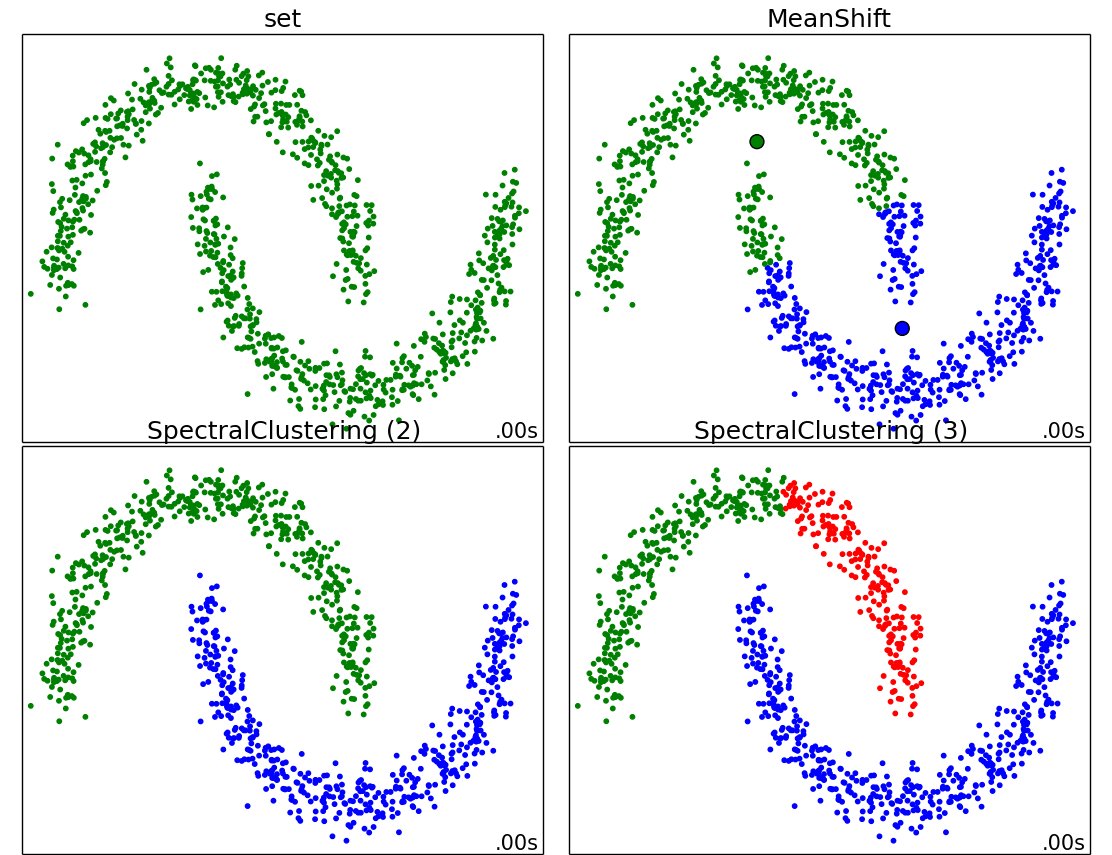
\includegraphics[width=8cm]{../pic/clustering_example_1.png}
	\end{center}
	\end{frame}
   
   \begin{frame}{Кластеризация}
   Если данные разряжены и/или их мало (например всего 100 точек), то кластеризация работает плохо:
   \begin{center}
   	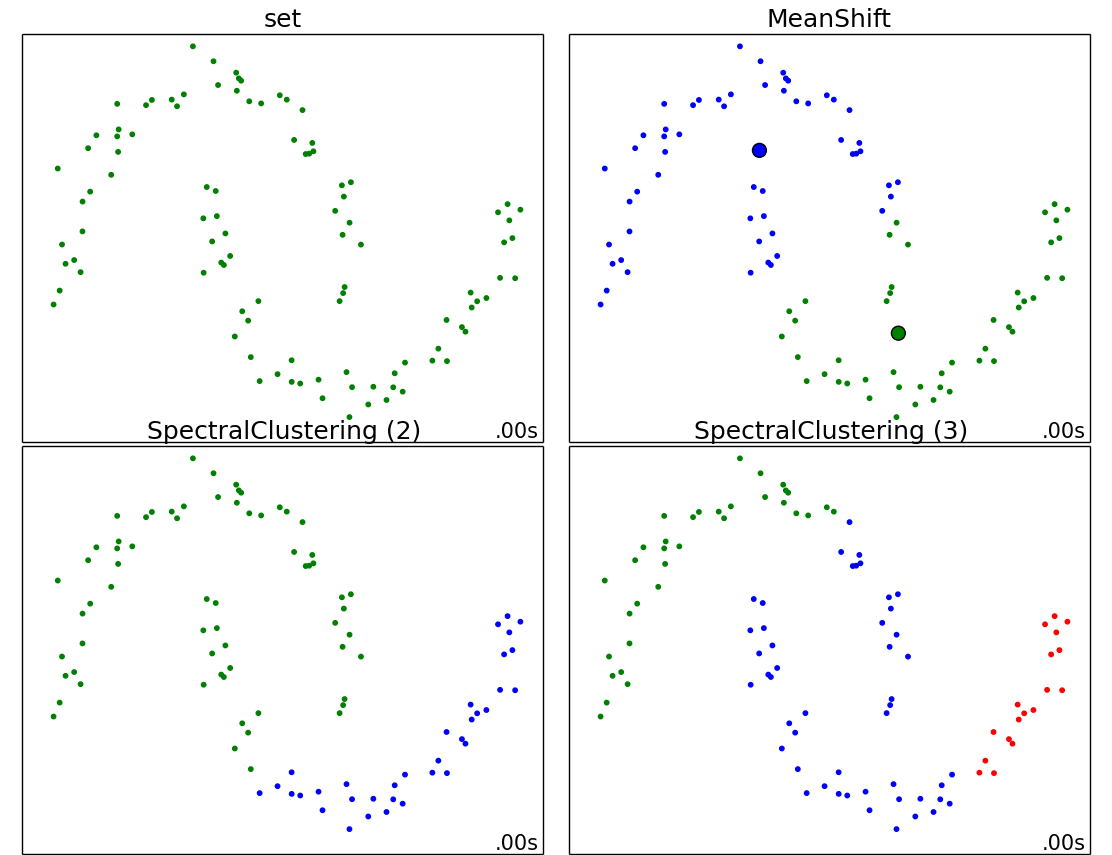
\includegraphics[width=8cm]{../pic/clustering_example_2.png}
   \end{center}
	\end{frame}

   \begin{frame}{Кластеризация}
   Не всегда кластеры несут какой-либо смысл.
	\begin{center}
		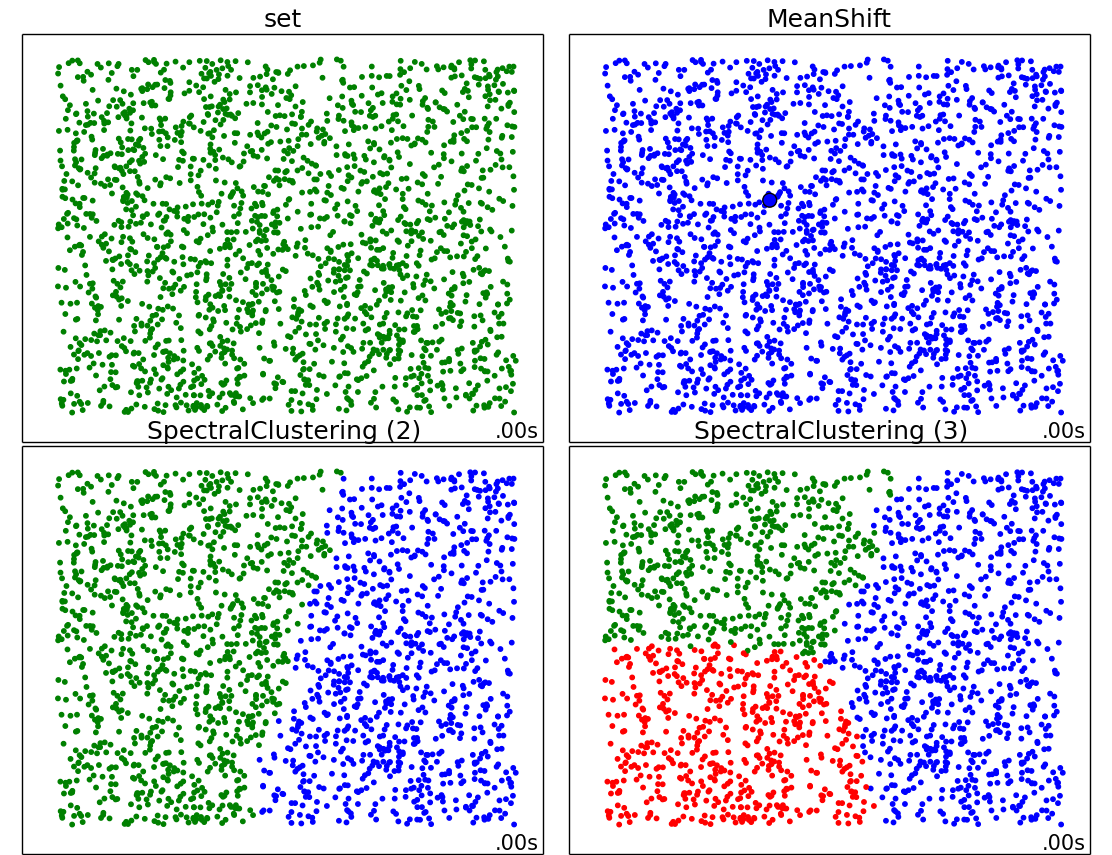
\includegraphics[width=8cm]{../pic/clustering_example_3.png}
	\end{center}
	\end{frame}

% TODO Доделать слайда
	\begin{frame}{Интерполяция}
	\termdef{Интерполяция} -- процесс нахождения промежуточных значений величины 
	$\hat {\bold x}$ 	
	по имеющейся совокупности её дискретных значений 
	$\{ \bold x, y\}$:
	
	\begin{equation}
	\hat y := fit(\{ \bold x, y\}; \hat {\bold x})
	\end{equation}
	\termdef{Регрессия} -- определение функции зависимости отклика $y$ от переменной $\bold x$ ... ... 
	\end{frame}
   
   \begin{frame}
   \termdef{Идентификация} -- установление тождественности неизвестного объекта известному на основании похожести или полного совпадения признаков.
   
   \end{frame}
   
   \section{Вопросы для самопроверки}

   \begin{frame}{Признаки, вектор признаков, выборка}
   \begin{enumerate}
   	\item Что такое \term{признак}?
   	\item Что такое несравнимый (категориальный) признак? Чем он отличается от сравнимого?
   	\item Что такое булевый признак? Числовой?
   	\item Приведите пример булевого и несравнимого признака. Болевого и сравнимого. 
   	\item Что такое \term{вектор признаков}? Есть два вектора $\bold x_a = (x_1, x_2)$ и $\bold x_b = (x_2, x_1)$.
   	Являются ли они идентичными? Можете привести задачу, когда являются?
   	\item Что такое \term{обучающая выборка}? Почему формула \eqref{eq:def_fit_sample} задаётся
   	как \textbf{неупорядоченная} совокупность, а не как список (т.е. упорядоченная совокупность).
   	Почему порядок перечесления данных в аргументе функции \eqref{eq:fit_def} не важен?
   \end{enumerate}
	\end{frame}

   \begin{frame}{Обучающая выборка со слайда №\ref{frame:class_feature_vector_example}}
 	Посмотрите на \term{выборку} со слайда №\ref{frame:class_feature_vector_example}. 
 	\begin{enumerate}
 	\item Верно ли утверждение, что если совершается оплата электроэнергии, то данная операция всегда легитимная?
 	\item Есть ли корреляция между возрастом клиента и мошенничеством при покупке авиабилетов? 
 	\item Можно ли предположить, что таксисты чаще обманывают молодых девушек? 
 	\item Покупает ли молодёжь авиабилеты через данный банк? 
 	\item Если совершают мошенничество в сфере автоперевозок, то обманывают мужчин или женщин?
	\end{enumerate}
	\end{frame}
  
  	\begin{frame}{Обучение и переобучение}
  		\begin{enumerate}
  			\item Что такое обучение (fitting)? Что такое переобучение? (overfitting)?
  			\item Почему функции $fit$ и $refit$ -- это функции высшего порядка?
  			\item Как с помощью ансамблирования уменьшить проблему переобучения (а для некоторых алгоритмов и вовсе его убрать) ?
  			\item можете предложить какую-либо меру измерить переобучение?
  			\item Верно ли утверждение, что чем больше и <<разнообразней>> выборка, тем меньше ошибок, вызванных переобучением?
  		\end{enumerate} 
	\end{frame}
  	
  	\begin{frame}{Полнота, точность и $coef_{fraud}$}
  		Существуют задачи, в которых физически невозможно рассчитать скоринг для всех 
  		мошеннических операций на определённом достаточном для анализа качества системы промежутке времени (например неделя).
  		К примеру -- это задача распознавания спама. Спама очень много...
  		
  		Тогда, для расчёта ${y, \hat y}$ выбирается лишь подмножество мошеннических операций для выборки $U_test$.
  		
  		Таким образом, аналогично $coef_{legitim}$ разумно определить коэфициент $coef_{fraud}$.
  		
  		Как тогда изменятся формулы \eqref{eq:recall_by_counts} и \eqref{eq:presicionl_by_counts}?
  		
  	\end{frame}
  
  	\begin{frame}{Задачи машинного обучения}
	\begin{enumerate}
		\item Чем классификация отличается от идентификации? Можно ли идентификацию назвать классификацией с большим количеством классов?
		\item Что такое кластеризация? Может ли кластеризация быть одним из предварительных действий для классификации? 
		\item Что такое регрессия, интерполяция и аппроксимация? В чем отличие?
		\item Что такое прогнозирование? Если прогнозируемая величина дискретна и ограничена, можно ли задачу прогнозирования свести к задачи классификации?
		\item задачу классификации, кластеризации или прогнозирования решает обученная нейронная сеть?	
	\end{enumerate}  	  	
	
	\end{frame}
  

\end{document}